\documentclass[a4paper]{article}

%% Language and font encodings
\usepackage[english]{babel}
\usepackage[utf8x]{inputenc}
\usepackage[T1]{fontenc}

%% Sets page size and margins
\usepackage[a4paper,top=3cm,bottom=2cm,left=3cm,right=3cm,marginparwidth=1.75cm]{geometry}

%% Useful packages
\usepackage{amsmath}
\usepackage{graphicx}
\usepackage[colorinlistoftodos]{todonotes}
\usepackage[colorlinks=true, allcolors=blue]{hyperref}
\usepackage{subfigure} 
\usepackage{float}

\title{Estereotipos de Género en las Revistas Brando y Ohlala}
\author{Diego Kozlowski - Fernando Gonzalez - Alfredo Rolla - Jorge Federico Cubells}

\begin{document}

\begin{figure}
\centering

\includegraphics[width=0.8\textwidth]{logos/dmuba.PNG}
\end{figure}

\maketitle

\section{Introducci\'on}

En \'epocas donde el rol de la mujer en la sociedad est\'a cambiando, y donde se plantea de manera constante la ruptura de estereotipos de g\'enero en todos los \'ambitos de vida en sociedad, nos propusimos investigar esta tem\'atica desde la \'optica de c\'omo los medios gr\'aficos abordan la perspectiva de g\'enero.\\
Los medios gr\'aficos son instrumentos poderosos para mantener y/o cuestionar las ideolog\'ias de g\'enero de nuestra sociedad, y nuestra hip\'otesis principal de trabajo es que las revistas orientadas al p\'ublico de cada g\'enero se sustancian en l\'exicos y t\'opicos diferenciados.\\
\linebreak
El \textbf{Objetivo General} de este trabajo de investigaci\'on es "Analizar los estereotipos presentes en las revistas de consumo masivo y su evoluci\'on en los \'ultimos 10 a\~nos, mediante t\'ecnicas de procesamiento de lenguaje."\\
\linebreak
Los \textbf{Objetivos Espec\'ificos} son:
\begin{enumerate}
	\item Topic Modeling
		\begin{itemize}
		\item Construir un modelo de TM con el corpus completo (ambas revistas) para todos los a\~nos.
        \item Seleccionar t\'opicos que resulten de inter\'es a la investigaci\'on.
        \item Analizar la participaci\'on de cada uno de estos t\'opicos en cada revista en el tiempo.
		\end{itemize}
	\item Palabras / Listado de Palabras
		\begin{itemize}
		\item Realizar una selecci\'on de palabras que resulte de inter\'es seguir.
        \item Ver la evoluci\'on de la presencia de estas palabras en el tiempo, de forma condicional a cada revista.
        \item Analizar si la probabilidad de encontrar esas palabras condicionadas a cada revista es significativamente diferente para cada corpus.
        \item Comparar con hitos hist\'oricos relacionados.
\end{itemize}
\end{enumerate}

Las \textbf{Hip\'otesis de Trabajo} utilizadas son:
\begin{enumerate}
\item A lo largo del per\'iodo bajo an\'alisis, se mantiene la separabilidad de los corpus de cada revista por t\'opicos estereotipados, es decir que no refieren a diferencias genuinas entre el hombre y la mujer.
\item No obstante la hip\'otesis 1, existe un movimiento en el tiempo, donde desaparecen ciertos t\'opicos de contenido m\'as marcadamente mis\'ogino y aparecen ciertos t\'opicos nuevos, que expresan la superaci\'on de tab\'ues. 
\item Otros t\'opicos se mantienen en el tiempo, asignando roles aspiracionales diferenciados entre hombres y mujeres. Por ejemplo, como t\'opicos relevantes para los hombres los "negocios" y el "consumo suntuario" (aspiraciones econ\'omicas), y en la revista de mujeres se promueve la pseudociencia, como el "Hor\'oscopo", marcando una diferenciaci\'on respecto a las formas de "superaci\'on personal".
\end{enumerate}

\section{Metodolog\'ia}

El software utilizado para las tareas de obtenci\'on y procesamiento de los datos fue Python 3 \cite{python}.\\
Dentro del software citado, las principales librer\'ias utilizadas fueron:\\
\begin{itemize}
\item Pandas: para manejo de datos. \cite{pandas}
\item Numpy: de c\'alculos cient\'ificos para manejo de datos multidimensionales. \cite{numpy}
\item Scikit Learn: especializada en machine learning \cite{scikit}.
\item NLTK: para trabajar con datos del lenguaje natural. \cite{nltk}
\item Gensim: software robusto y eficiente para realizar modelado sem\'antico no supervisado a partir de textos \cite{gensim}.

\end{itemize}

La f\'ormula para el cálculo de la probabilidad de aparici\'on de una palabra dada un a revista es:\\
\begin{center}
$\text{P}[W_i|R_j] = \dfrac{\#W_{ij}}{\#W_{*j}}$
\end{center}
$W_i:$ Palabra en particular.\\
$\#W_{ij}:$Total de esa palabra para esa revista. \\
$\#W_{*j}:$Total de palabras en el corpus para esa revista.\\
$R_j:$ Revista j.\\

La f\'ormula para el cálculo de la probabilidad de aparici\'on de un t\'opico dada una revista es:\\
\begin{center}
$\text{P}[T_i|R_j] = \dfrac{\sum_{d=1}^{d=m} P(T_{ijd})}{\#d}$
\end{center}
$T_i:$ T\'opico en particular.\\
$P(T_{ijd}):$ Probabilidad del t\'opico i para la revista j para el documento d.\\
$\#d:$ N\'umero de documentos.\\
$R_j:$ Revista j.\\

%Para realizar la evaluación de la significancia estad\'istica de la asociación entre t\'opicos de las revistas se empleo el test de Mann-Whitney-Wilcoxon, test no param\'etrico de diferencia de medias.\\

Para realizar la evaluación de la significancia estadística de la asociación entre las revistas, en el caso del an\'alisis de  palabras y listas de palabras por años, se empleó el test exacto de Fisher, que permite testear dicha significancia a partir de una tabla de contingencia.\\

\section{Selecci\'on y Limpieza del Corpus}

Para la realizaci\'on de este trabajo se utilizaron dos revistas disponibles online, cuyo target de p\'ublico es respectivamente el colectivo masculino y femenino.\\

\subsection{Selecci\'on y Obtenci\'on del Corpus}
Tanto Ohlala como Brando son revistas del Diario La Naci\'on que se encuentran disponibles online.\\
Debido a que busc\'abamos con este trabajo detectar la evoluci\'on de los t\'opicos y palabras a lo largo de los a\~nos, y teniendo en cuenta que ambas revistas se publican desde mediados de la d\'ecada del 2000, se procedi\'o a obtener los art\'iculos publicados.\\

\begin{figure}[H]
\centering
\subfigure[Brando]{
\includegraphics[width=30mm]{logos/brando.jpg}}
\subfigure[Ohlala]{
\includegraphics[width=50mm]{logos/OHLALA.png}}
\caption{Revistas de G\'enero} \label{fig:logos}
\end{figure}

La definici\'on fue tomar los art\'iculos de los \'ultimos 10 a\~nos para cada revista.\\
Para ello elaboramos un web scraper que incluye dos pasos principales:

\begin{enumerate}
\item \textbf{Obtenci\'on de las URLs}: Se hizo un an\'alisis inicial de la p\'agina web, a partir de la cual se detect\'o la existencia de una API interna en La Naci\'on. Dicha API permite ir navegando por los art\'iculos hist\'oricos de las revistas mediante el bot\'on "siguiente".\\
Los inputs de dicha API son:
	\begin{itemize}
	\item \textit{Magazine}: puede ser Brando, Ohlala, Hola, Lugares, Living, Jard\'in, Editorial y Tecnolog\'ia. Nosotros trabajaremos con las dos primeras.
	\item \textit{N\'umero de p\'agina (p)}: de la historia de los art\'iculos donde nos encontramos. Iniciamos en la p\'agina 1.
	\item \textit{N\'umero de art\'iculos a devolver en cada p\'agina (c)}: Seteado en 100 art\'iculos por p\'agina.
	\end{itemize}
\item \textbf{Obtenci\'on de los Documentos}: el resultado es un diccionario de python con la siguiente estructura:

\vspace{1mm} %5mm vertical space
\begin{center}
$\textbf{\textit{Url: [Magazine, Fecha, Titulo, Texto]}}$\\
\vspace{1mm} %5mm vertical space
\end{center}
Donde:\\
\textbf{Url}: Link al art\'iculo recuperado.\\
\textbf{Magazine}: Nombre de la revista.\\
\textbf{Fecha}: Fecha normalizada ISO-8601 (YYYY-MM-DD).\\
\textbf{T\'itulo}: T\'itulo del articulo, limpio de codigo html y caracteres especiales.\\
\textbf{Texto}: Texto del art\'iculo, limpio de codigo html y caracteres especiales.\\

\end{enumerate} 

Como resultado de este web scraping obtuvimos en principio 7.779 art\'iculos en Brando y 22.309 art\'iculos en Ohlala.

\begin{figure}[H]
\centering
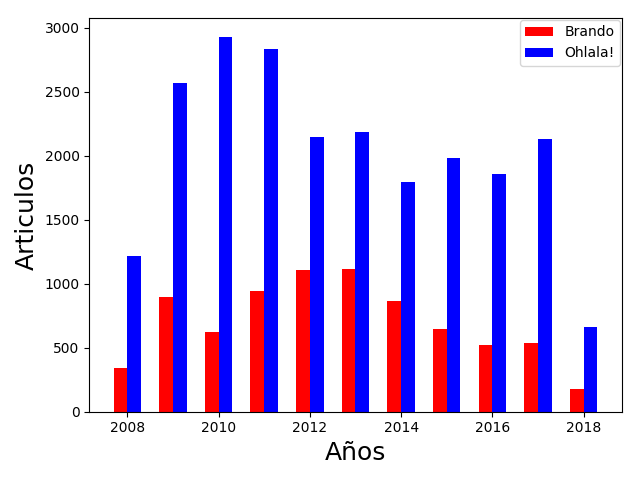
\includegraphics[width=0.5\textwidth]{graficos/articulosxrevista.png}
\caption{N\'umero de Art\'iculos por Revista} 
\end{figure}

Aclaramos que en principio ese es el n\'umero de revistas, ya que veremos que luego de la limpieza dicha cantidad se redujo considerablemente debido a la existencia de art\'iculos vac\'ios (ejemplos: encuestas, im\'agenes sin texto,etc.).

\subsection{Limpieza del Corpus}

Los pasos seguidos fueron:
\begin{enumerate}
\item \textbf{Carga y Join de Corpus}: Se leyeron los corpus de Brando y Ohlala y luego se realiz\'o el join.
\item \textbf{Normalizaci\'on de Fechas}: Solamente nos interesa el a\~no de publicaci\'on de cada art\'iculo, por lo tanto, se extrajo dicha informaci\'on de las fechas y se la incorpor\'o como feature.
\item \textbf{Limpieza}:
	\begin{itemize}
	\item Se armaron dos listados, uno de palabras y otro de frases, que ser\'ian exlu\'idos del corpus. Las palabras son aquellas ambiguas y comunes en nuestro lenguaje, y otras que pueden sesgar el an\'alisis (ejemplo ohlaleando, brando). Las frases son especialmente Disclaimers que aparec\'ian al final de la mayor\'ia de los art\'iculos (ejemplo: "Los comentarios publicados son de exclusiva responsabilidad de sus autores...", "Enviar un comentario implica la aceptación del Reglamento.").
    \item Eliminaci\'on de Stopwords del Espa\~nol.
    \item Remoci\'on de acentos. 
    \item Reemplazo de signos de puntuaci\'on por un espacio. Esto es as\'i porque de no incluir el espacio hac\'ia que las palabras se unieran.
    \item Llevar a min\'usculas todas las palabras.
    \item Reemplazo de todos los valores num\'ericos por la palabra "NUM".
	\end{itemize}
\item \textbf{Stemming}: recorte de las palabras de manera de generalizarlas. Ejemplo: Biblioteca y Bibliotecario a Bibliotec
\item \textbf{Destemming}: Implica llevar cada "stemm" a una palabra que tenga m\'as sentido al leerla. Esto se hace asignando la palabra completa que mayor frecuencia tenga en cada stemm. Bibiotec a Biblioteca, asumiendo que esta aparece con mayor frecuencia que Bibliotecario. 
\item \textbf{Eliminaci\'on de Art\'iculos Vac\'ios}: el total de art\'iculos se reduce de cerca de 30 mil a 24.142, repartidos en 6.060 art\'iculos en Brando y 18.082 en Ohlala.
\begin{figure}[H]
\centering
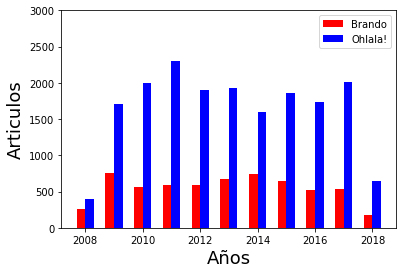
\includegraphics[width=0.5\textwidth]{graficos/corpus_20k.png}
\caption{N\'umero de Art\'iculos por Revista post Limpieza} 
\end{figure}
\end{enumerate}

Como un primer an\'alisis exploratorio buscamos conocer cu\'ales eran las palabras que mejor distingu\'ian a cada revista.\\
Para ello armamos una wordcloud por revista, filtrando aquellas palabras con una probabilidad mayor a 0.001 y con un odd superior a 2.\\
\linebreak
Definimos odd como el cociente entre la probabilidad que la palabra $W_{i}$ aparezca en la Revista 1, dividido la probabilidad que dicha palabra aparezca en la Revista 2.\\

\begin{center}
$\text{Odd} = \dfrac{P (W_i | Revista_1)}{P (W_i | Revista_2)}$
\end{center}


\begin{figure}[H]
\centering
\subfigure[Brando]{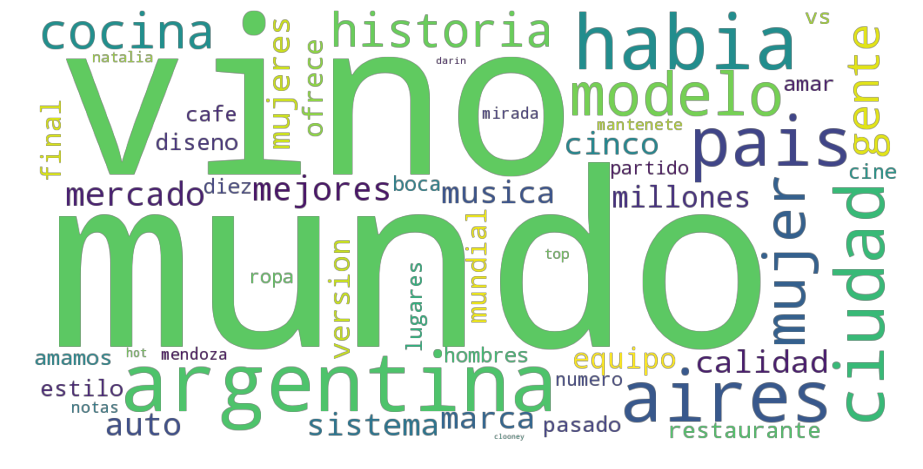
\includegraphics[width=70mm]{graficos/wordcloud_brando.png}}
\subfigure[Ohlala]{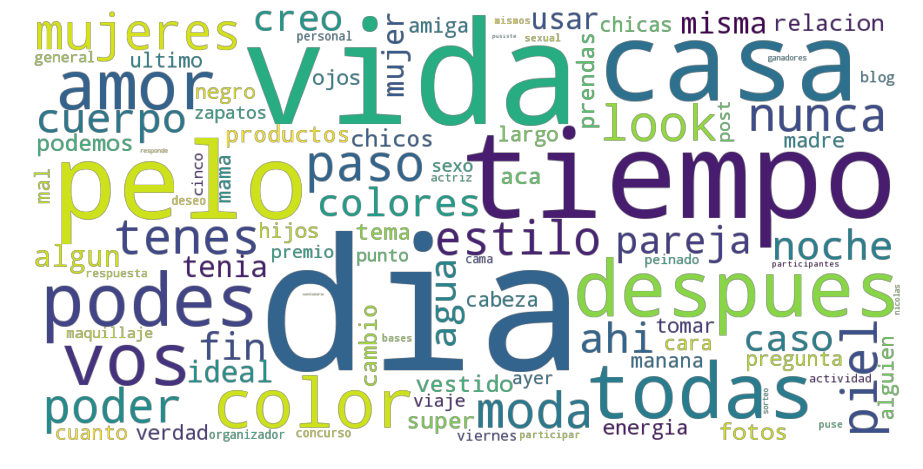
\includegraphics[width=70mm]{graficos/wordcloud_ohlala.png}}
\caption{Wordcloud por Revista. Palabras que distinguen} \label{fig:wordcloud}
\end{figure}

Notamos que en el caso de la revista masculina, las palabras que la distinguen son Vino, Mundo, Modelo, Argentina, Ciudad, Gente, Cocina, Auto, Sistema, Equipo, Marca, Mujer/es entre otras.\\
Para el caso de la revista femenina son Vida, D\'ia, Tiempo, Pelo, Casa, Color, Moda, Podemos, Todas, Amor, Piel, entre otras.\\
Es pertinente aclarar que la palabra "vs" (abreviaci\'on de versus) aparece seguido en articulos anteriores a 2011 en Brando, y proviene de notas cuya tematica era la comparaci\'on de modelos mujeres. Esto se evidencia con la aparicion de palabras como "hot", "mujeres" y "modelo" en el wordcloud.\\
Esto nos da pautas de los temas que se podr\'ian estar tratando en ambas revistas, con algunos m\'as relacionados a Autos, Negocios, Sociedad y Pol\'itica, Tecnolog\'ia (Brando), y otros m\'as relacionados a Moda, Cuidado Personal, Casa y Familia (Ohlala).


\section{An\'alisis de T\'opicos}

\subsection{Aplicaci\'on del Modelo}
Para detectar los t\'opicos del corpus se aplic\'o el modelo estad\'istico generativo denominado Latent Dirichlet Allocation (LDA) desarrollado por David Blei et al (2003) \cite{LDA}.\\
Con este modelo a partir de la matriz T\'ermino-Documento se obtuvieron dos matrices: la matriz T\'ermino-T\'opicos y la matriz T\'opicos-Documentos. En la primera tendremos la distribuci\'on de las palabras en los distintos t\'opicos y la segunda la distribuci\'on de los t\'opicos en los documentos.\\
Los par\'ametros usados por este modelo son:
\begin{itemize}
\item \textit{Input}: corpus luego de la limpieza.
\item \textit{M\'aximo de Iteraciones}: se defini\'o en 50.
\item \textit{M\'etodo de Aprendizaje}: seteado en "Online" que se corresponde al M\'etodo Variacional Bayesiano.
\item \textit{Semilla}: se defini\'o una semilla para que arroje los mismos resultados para poder repetir los experimentos.
\item \textit{N\'umero de T\'opicos}: definido en 100 t\'opicos.
\end{itemize}

Una vez entrenado el modelo, se lo aplic\'o sobre el corpus para obtener las matrices T\'ermino-T\'opicos y T\'opicos-Documentos.
Con este procedimiento pudimos  conocer qu\'e t\'opicos son tratados en cada documento de las revistas, y cu\'ales son las palabras m\'as representativas de cada uno de los 100 t\'opicos.

\subsection{Resultados}
	\subsubsection{T\'opicos Relevantes}
    Analizando las 10 palabras m\'as importantes de cada t\'opico, y atendiendo a las hip\'otesis de trabajo definidas, seleccionamos 9 t\'opicos.
    
    \begin{table}[!htbp]
	\centering
	\begin{tabular}{|p{1cm}|p{2cm}|p{10cm}|}
\hline
Nro T\'opico & Nombre Asignado & Top 10 Palabras\\
\hline
1 & Objetivaci\'on Mujer & natalia hot ana emma romina versus diez camilo morochas mega\\
4 & Negocios & empresa redes sistema comprar productos mercado traves tecnologia permite desarrollo\\
5 & Autos & version auto marca modelo presente equipo llego motor argentina electrica\\
7 & Ni\~nos & ninos adultos educativo colegio chiquito padre secuestro change sauna pegote\\
%9 & Vinos & vino dulce bebe elaborado bodega sabor frutas aromas mejores botella\\
21 & Moda & moda diseno estilo marca coleccion ropa tendencia prendas rosa zapatillas\\
%24 & M\'usica & musica canciones disco banda video tema rock bailar cantar musical\\
%27 & Sexo & mujeres hombre sexo pareja sexual masculino deseo placer fantasia erotica\\
50 & Familia & hijos madre mama padre bebe familia papa embarazo regalo anos\\
71 & Sociedad & anos argentina mundo historia pais publico primera habia libro mundial\\
82 & Investigaci\'on & estudio problema trabajo explica ley medico social generar desarrollo investigar\\
%87 & Educaci\'on & clases curso aprender estudio taller enseno labial alumnos profesor docente\\
%88 & Cocina & cocina queso com recetas platos carne cafe pan leche sabor\\
93 & F\'utbol & juego jugar futbol cancha programa ganas copa radio pelota gol\\
\hline


\end{tabular}
\caption{\label{tab:widgets}T\'opicos Seleccionados}
\end{table}

\subsubsection{Evoluci\'on en el Tiempo}

\begin{figure}[H]
\centering
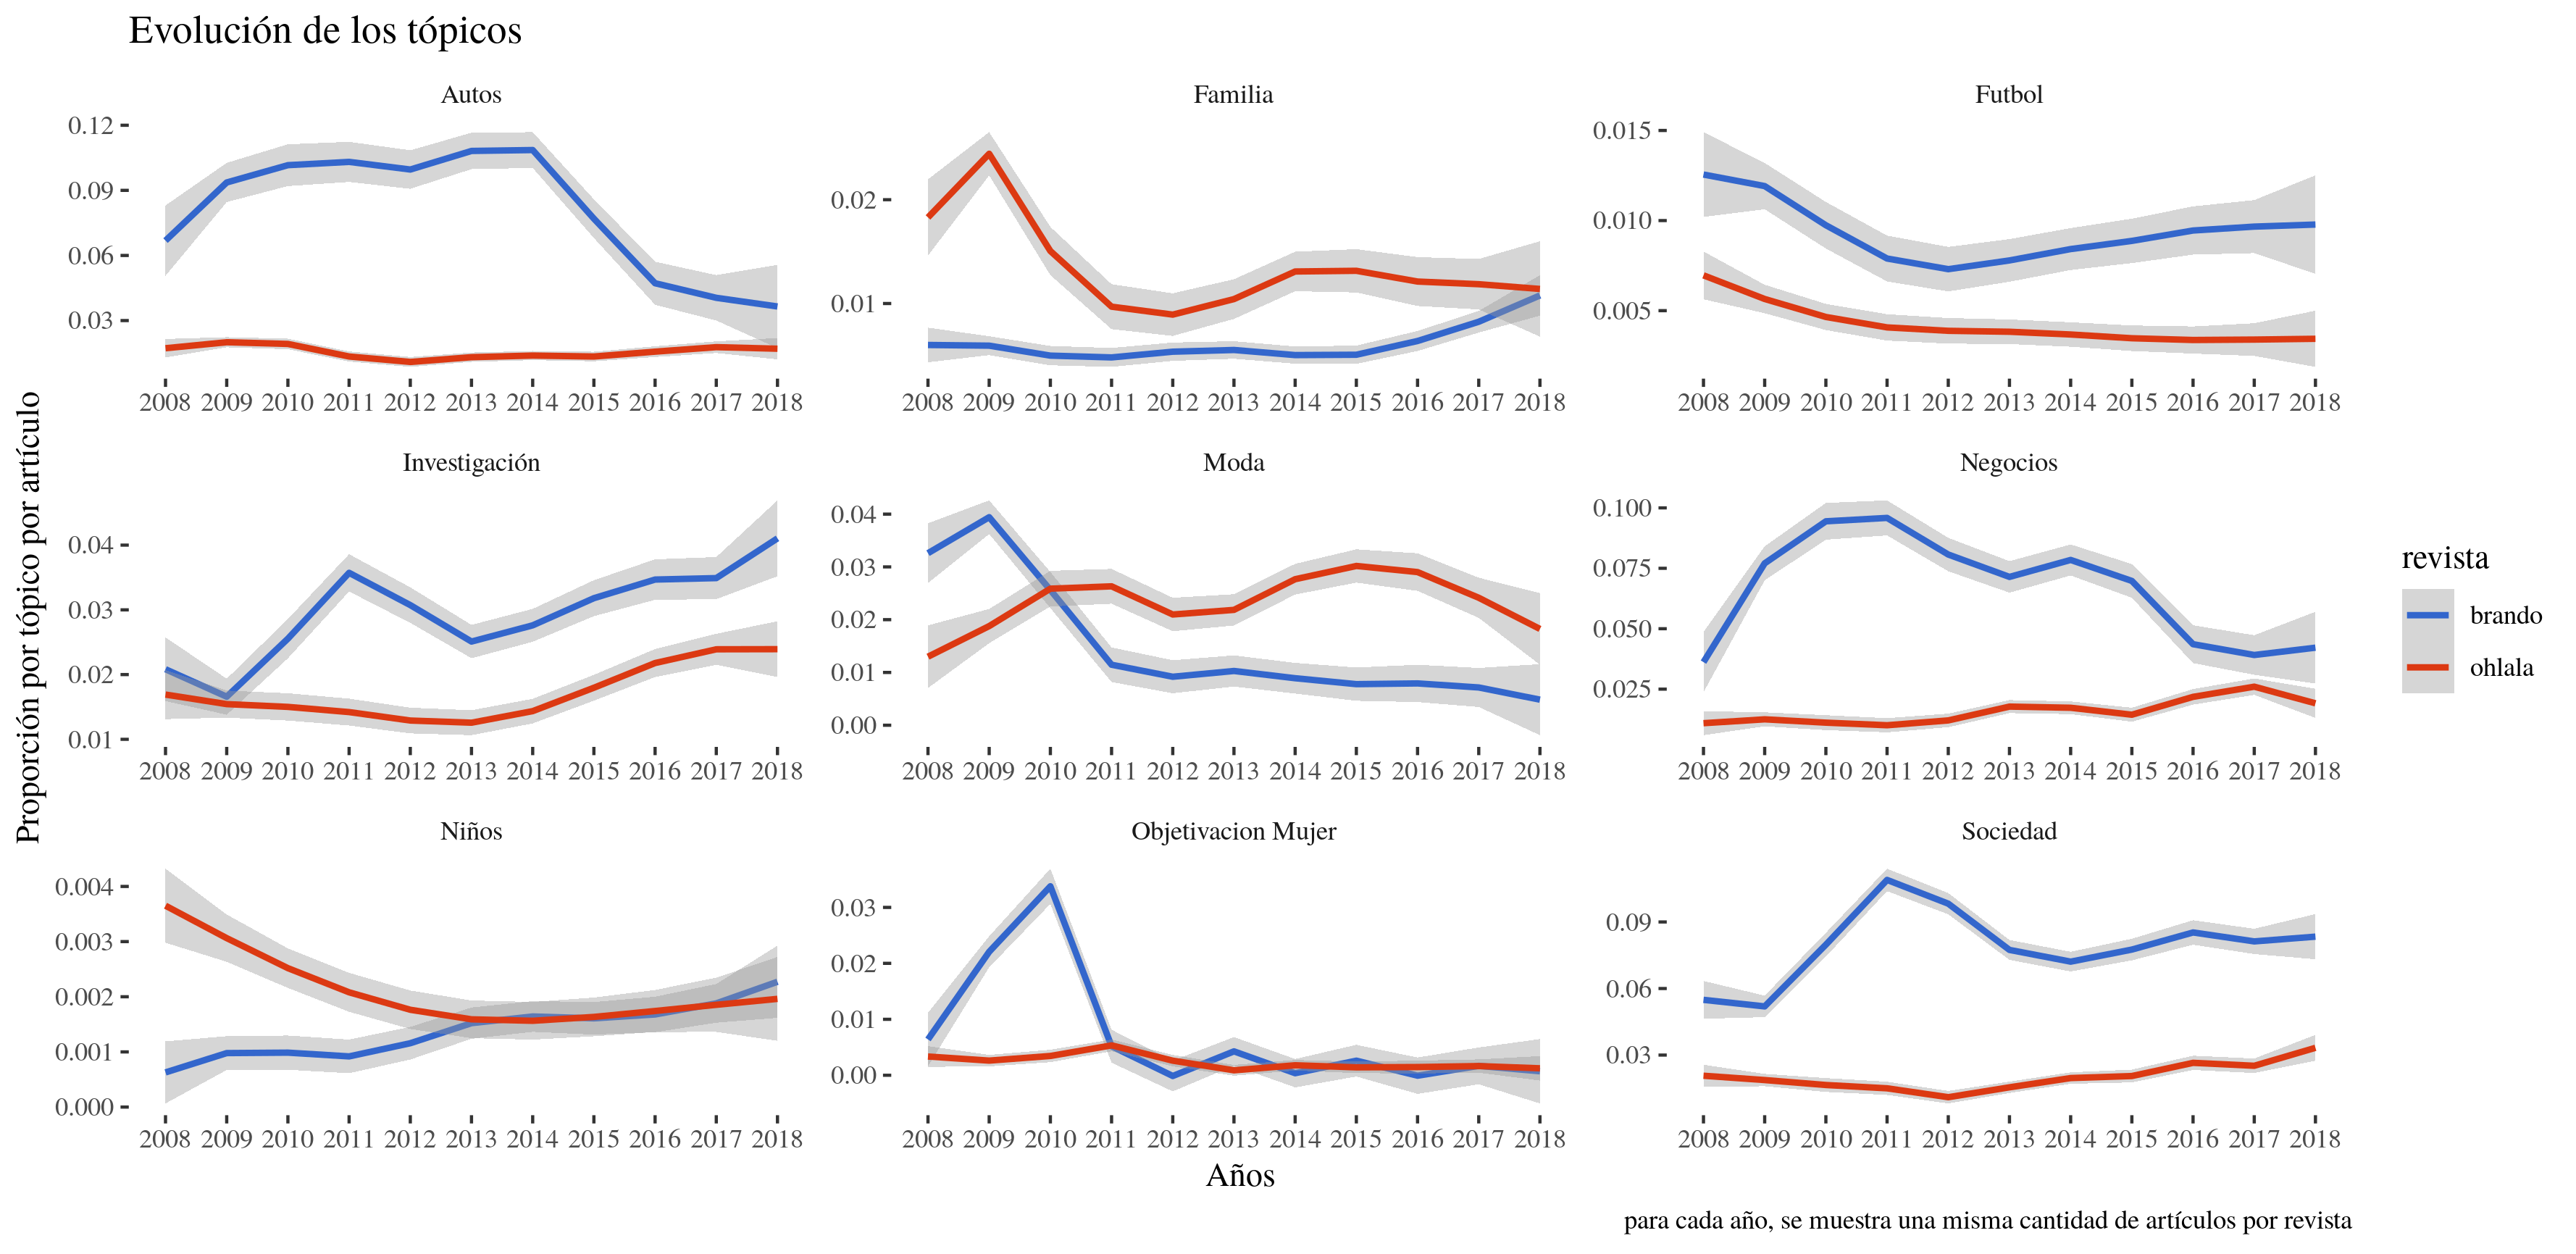
\includegraphics[width=1\textwidth]{graficos/evol_topicos_smooth.png}
\end{figure}

En cuanto al t\'opico \textbf{"Objetivaci\'on de la Mujer"} notamos que claramente a los inicios de ambas revistas, Brando utilizaba este t\'opico en mayor proporci\'on que Ohlala. Aunque tambi\'en notamos que a partir de 2012 los niveles bajaron considerablemente, quiz\'as con un cambio editorial acorde a las nuevas \'epocas.\\

El t\'opico de \textbf{"Ni\~nos"} estaba claramente mayor representado en Ohlala, como una tem\'atica de mayor inter\'es para las mujeres. Sin embargo hacia 2013 se nota que las proporciones de este t\'opico en ambas revistas se asemeja, incluso toc\'andose en mayor medida en Brando a partir de 2017.

Los t\'opicos \textbf{"Negocios"}, \textbf{"Futbol"} y \textbf{"Sociedad"} son mayormente tratados en Brando a lo largo del tiempo. Sin embargo en Negocios vemos c\'omo la proporci\'on en Brando cae de niveles de 0.075 a 0.040, aunque a\'un por encima de Ohlala.
Suponemos que Negocios es un t\'opico mayormente abordado en Brando porque se asocia al hombre con emprendedor, hombre de negocios. Con lo cual en principio se ver\'ia corroborada la hip\'otesis 3.
Las tem\'aticas asociadas a "Sociedad" (pol\'itica, historia, etc.) tambi\'en se tocan m\'as en Brando, probablemente asociado al estereotipo de hombre como principal actor en la vida pol\'itica y social de un pa\'is.
Y finalmente Futbol con marcada tendencia masculina, asumiendo una preferencia por este deporte por encima de las mujeres.\\

Cabe resaltar el comportamiento del t\'opico \textbf{"Familia"}. Durante la historia es mayormente tratado en la revista femenina, aunque vemos que en 2018 dicha diferencia de proporciones desaparece. La familia pasa de ser un tema poco tocado en Brando (valores cercanos a 0.005) a un tema que comienza a incorporarse a la l\'inea editorial (0.011). Aqu\'i podr\'ia estar indicando el cumplimiento de las hip\'otesis 1 y 2, ya que la familia era m\'as asociada a la mujer (rol de madre, ama de casa) pasando luego a ser un tema cada vez m\'as compartido (se observa el movimiento en el tiempo planteado en H3).\\

Dos temas marcadamente de preferencia de cada uno de los g\'eneros son los \textbf{"Autos"} para los hombres y la \textbf{"Moda"} para las mujeres (aunque aqu\'i vemos que a los inicios entre 2008 y 2010 era un tema mayormente tocado por la revista de hombres).\\

EL t\'opico asociado a \textbf{"Investigaci\'on"} ha visto incrementada su participaci\'on en ambas revistas a lo largo de los a\~nos, aunque la brecha entre la revista de hombres y mujeres tambi\'en se hizo mayor.


\section{An\'alisis de Palabras y Listas de Palabras}

\subsection{Selecci\'on de Palabras/Listado de Palabras}

Para la selecci\'on del listado de palabras a observar en cada revista y en el tiempo, nos basamos en:

\begin{enumerate}
\item Listados de Palabras en p\'aginas web que hablaran sobre los temas que nos interesaban para este trabajo
\item Listados elaborados por el equipo de investigaci\'on
%\item Listados extra\'idos de papers sobre tem\'atica de g\'enero
\end{enumerate}

Para la tem\'atica \textbf{"Feminismo"} elegimos los listados de palabras de los links:
\begin{itemize}
\item Diccionario Feminista \cite{diccfeminista}
\item Feminismo de la 'A' a la 'Z' \cite{feminismoaz}
\item Glosario feminista para principiantes \cite{glosariofemin}
\end{itemize}
All\'i encontramos palabras como Cosificaci\'on, Machismo, Micromachismo, Falocentrismo, Feminismo, entre otras.\\

Para la tem\'atica \textbf{"Sexista"} o maneras machistas de referirse a las mujeres el link usado fue de "Lenguaje Sexista para describir mujeres" \cite{machismo}.Las palabras relevantes son por ejemplo Bruja, Frigida, Puta, entre otras.\\

En cuanto a \textbf{"Ciencia"} consultamos la p\'agina web "100 palabras relacionadas con tecnolog\'ia" \cite{tecnologia} con palabras como Algoritmo, Cient\'ifico, Computaci\'on, Econom\'ia, entre otras.\\

Para el grupo de palabras relacionadas a \textbf{"Negocios"} consultamos el art\'iculo "Diccionario emprendedor ¡50 t\'erminos que debes conocer!" \cite{negocios} con palabras como Capital, Riesgo, Emprendedor, Marketing, Innovacion, entre otras.\\

Para lo \textbf{"Trendy"} o tendencia, elaboramos un listado propio con t\'erminos como Tablet, Iphone y Gaming.\\

Para \textbf{"Moda"} usamos el art\'iculo "Diccionario de palabras utilizadas en la moda" \cite{moda} con palabras como Escote, Chic y Outfit.\\

Otra tem\'atica de inter\'es es \textbf{"Hor\'oscopo}, donde en un listado de elaboraci\'on propia incluimos palabras como Hor\'oscopo, y los signos del sod\'iaco como Tauro, Aries y G\'eminis.\\

Finalmente para los \textbf{"Tab\'ues"} elaboramos un listado propio, con t\'erminos como Masturbaci\'on, Orgasmo, Menstruaci\'on y Swinger.\\


%Del paper de Marisol del-Teso-Craviotto \cite{women_magazines} extrajimos palabras comunmente utilizadas en las revistas estadounidenses Good Housekeeping, Cosmopolitan, Working Woman y Ms. para verificar si eran tambi\'en utilizadas en Ohlala (en mayor medida que en Brando).

%GH: Familia: Hijo, Hija, Ni\~no, Ni\~na, Madre, Familia, Esposo, Casarse 

\subsection{Evoluci\'on en el Tiempo}

\begin{figure}[H]
\centering
\subfigure[Ciencia]{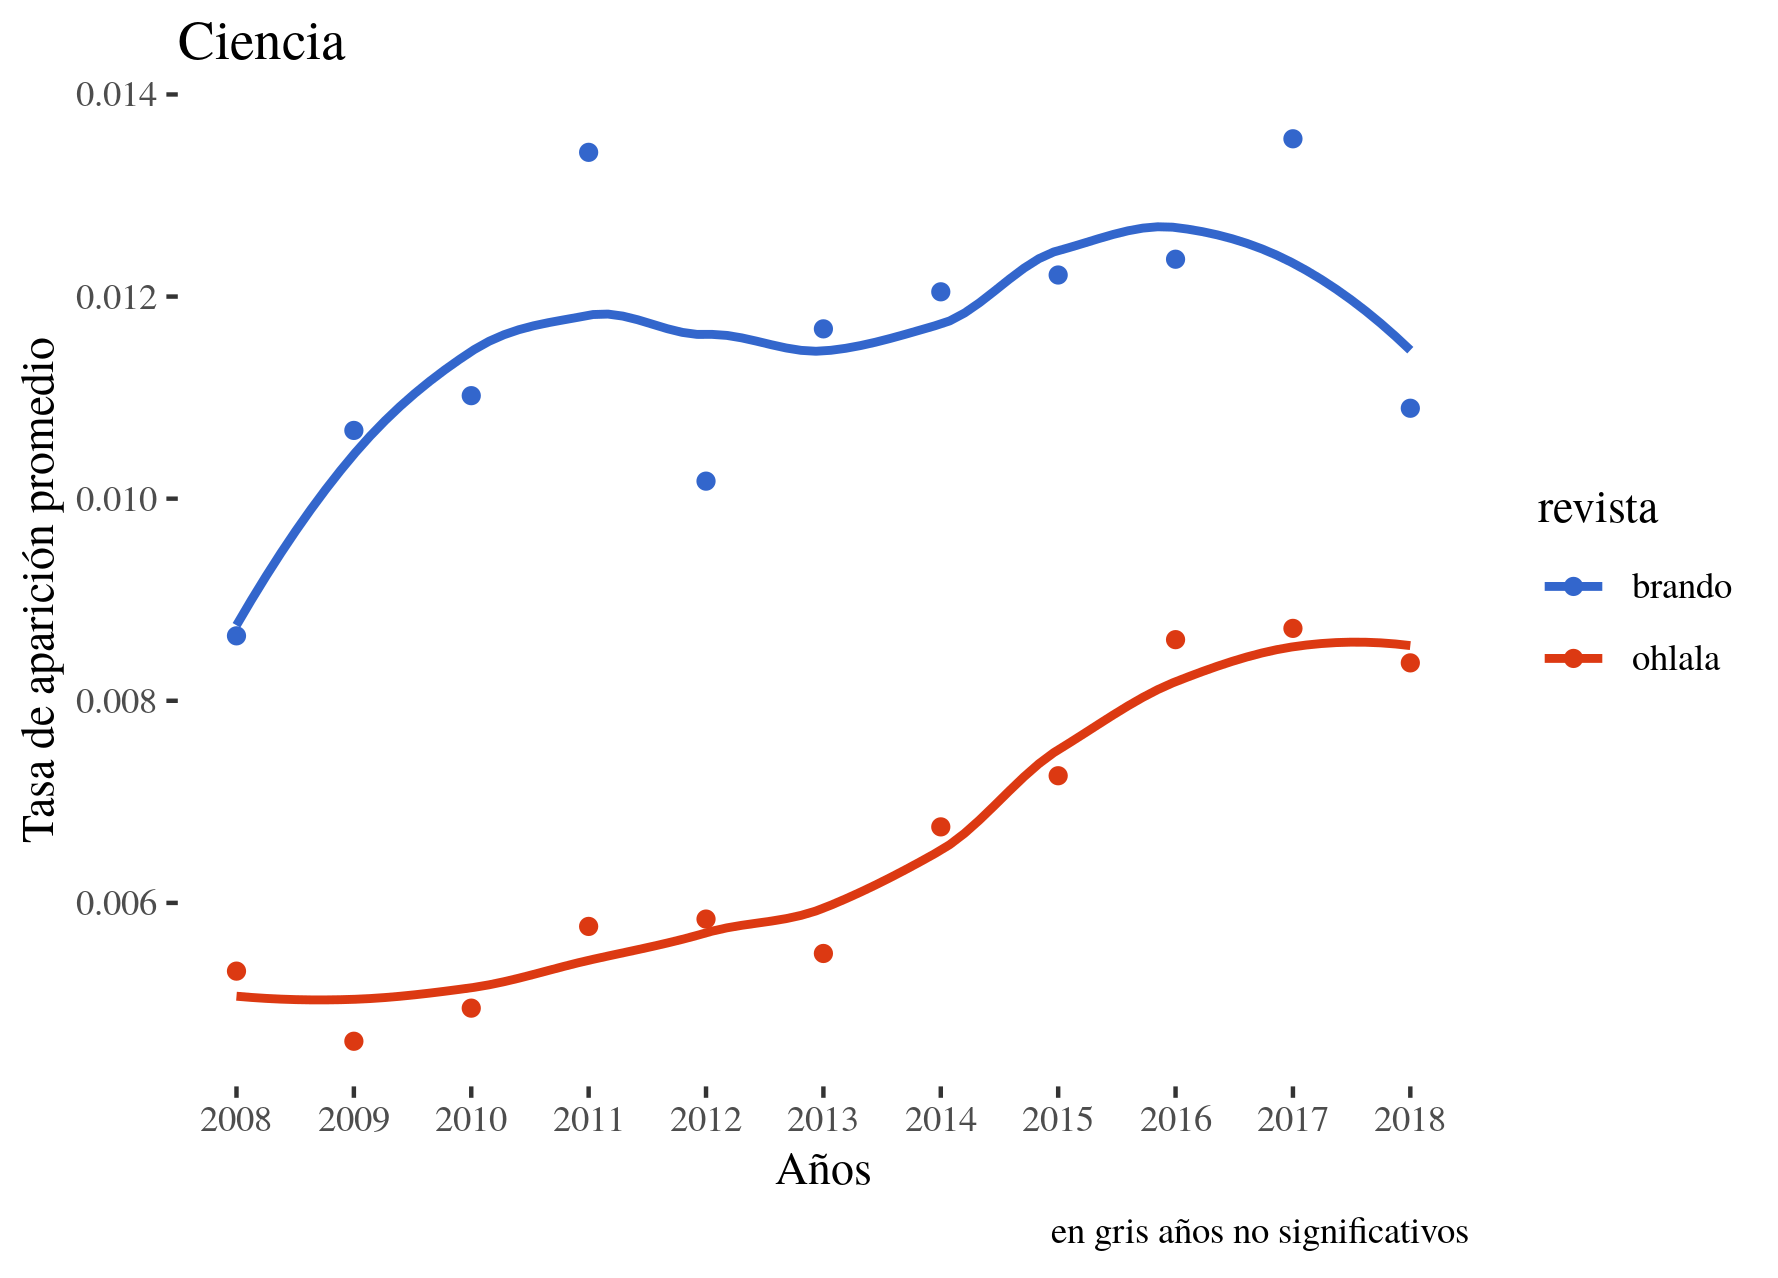
\includegraphics[width=65mm]{graficos/Ciencia.png}}
\subfigure[Trendy]{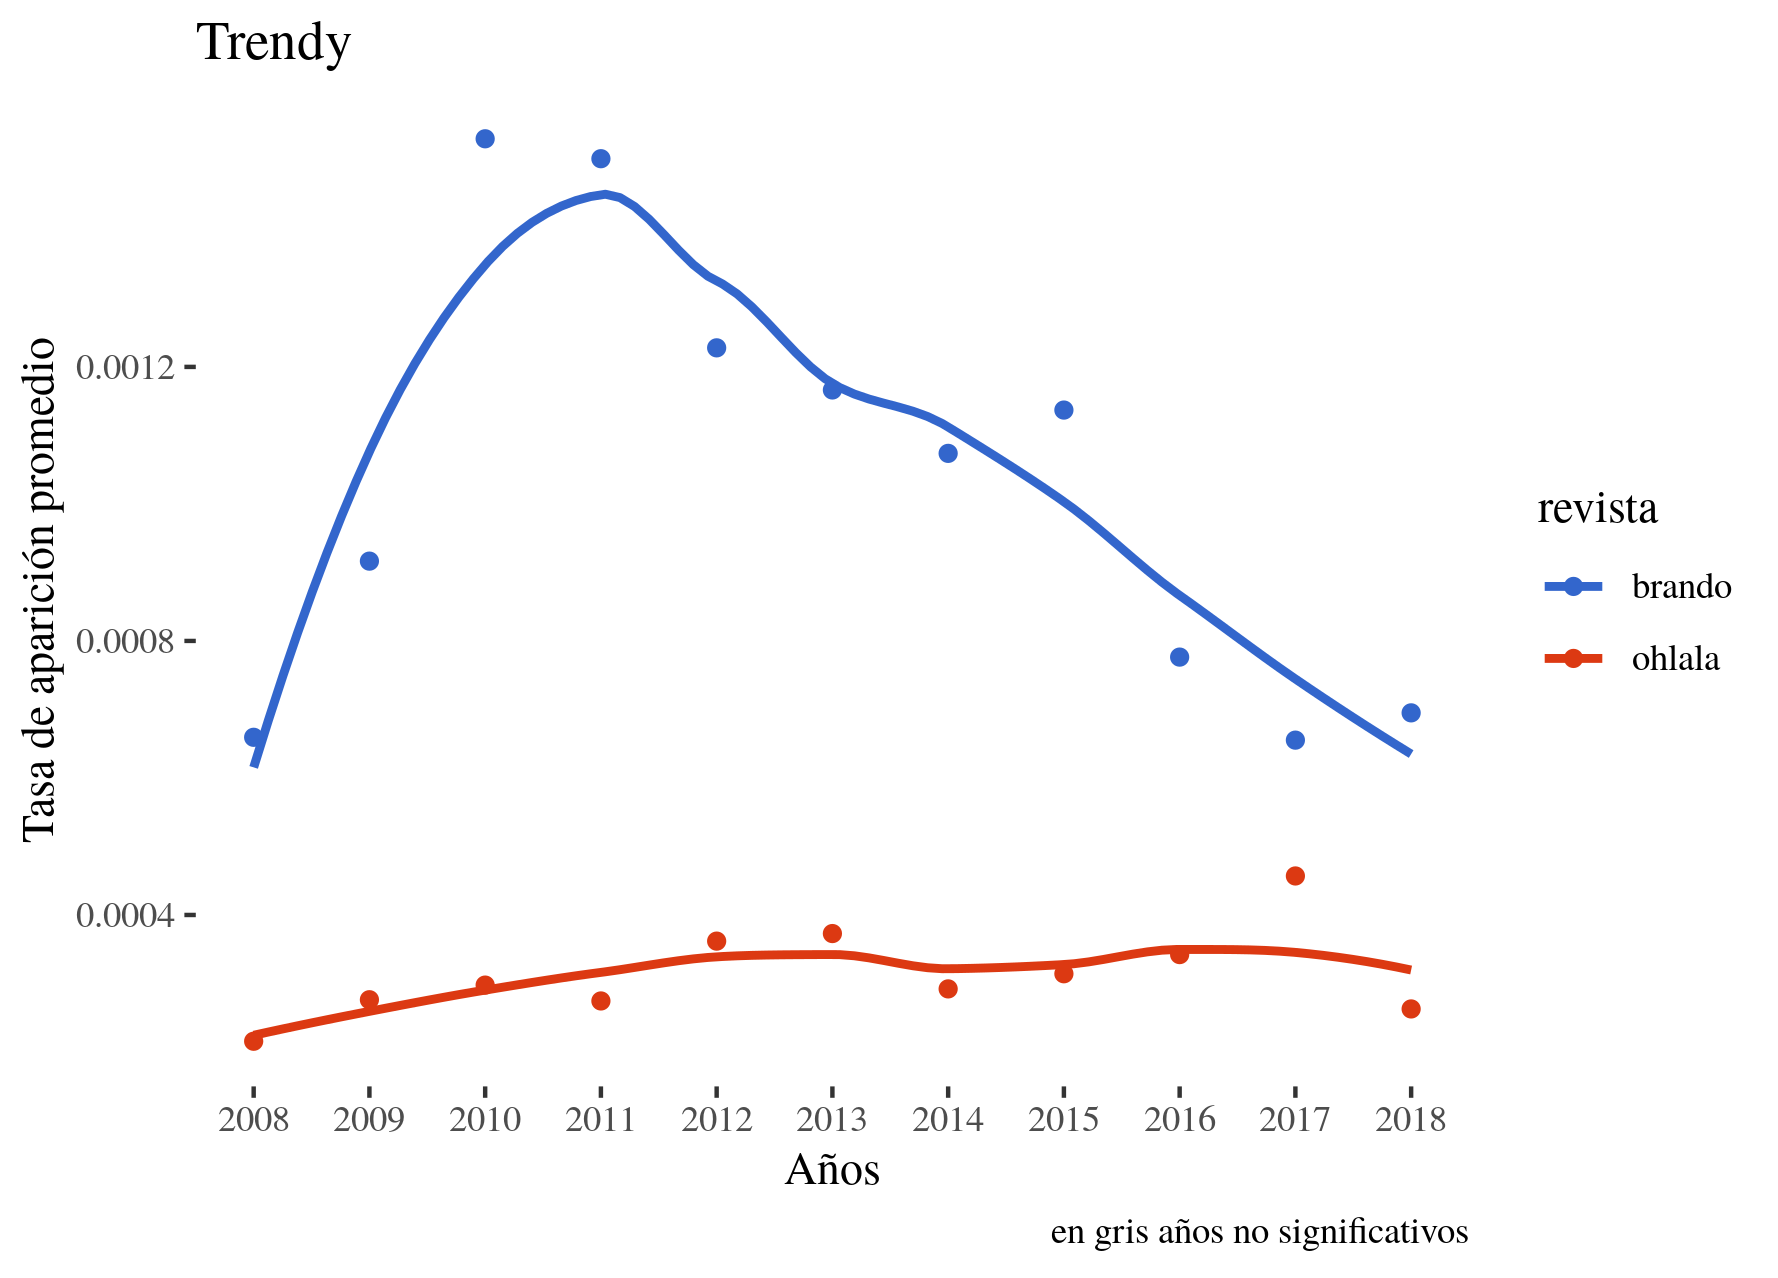
\includegraphics[width=65mm]{graficos/Trendy.png}}
\caption{Palabras relacionadas a Ciencia y Trendy} \label{fig:cienciaytrendy}
\end{figure}

En cuanto a las palabras asociadas a \textbf{"Ciencia"} y \textbf{"Trendy"} notamos que son mayormente utilizadas en la revista de orientaci\'on masculina con una diferencia significativa a lo largo de los a\~nos.\\
Sin embargo, la revista de orientaci\'on femenina comenz\'o a utilizar l\'exico asociado a Ciencia, con lo cual podr\'iamos estar ante evidencia de deconstrucci\'on de estereotipos, d\'andole m\'as relevencia a estos temas para las mujeres (H2).\\
Las palabras asociadas a Trendy est\'an us\'andose en menor proporci\'on a lo largo de los a\~nos en Brando.

\begin{figure}[H]
\centering
\subfigure[Moda]{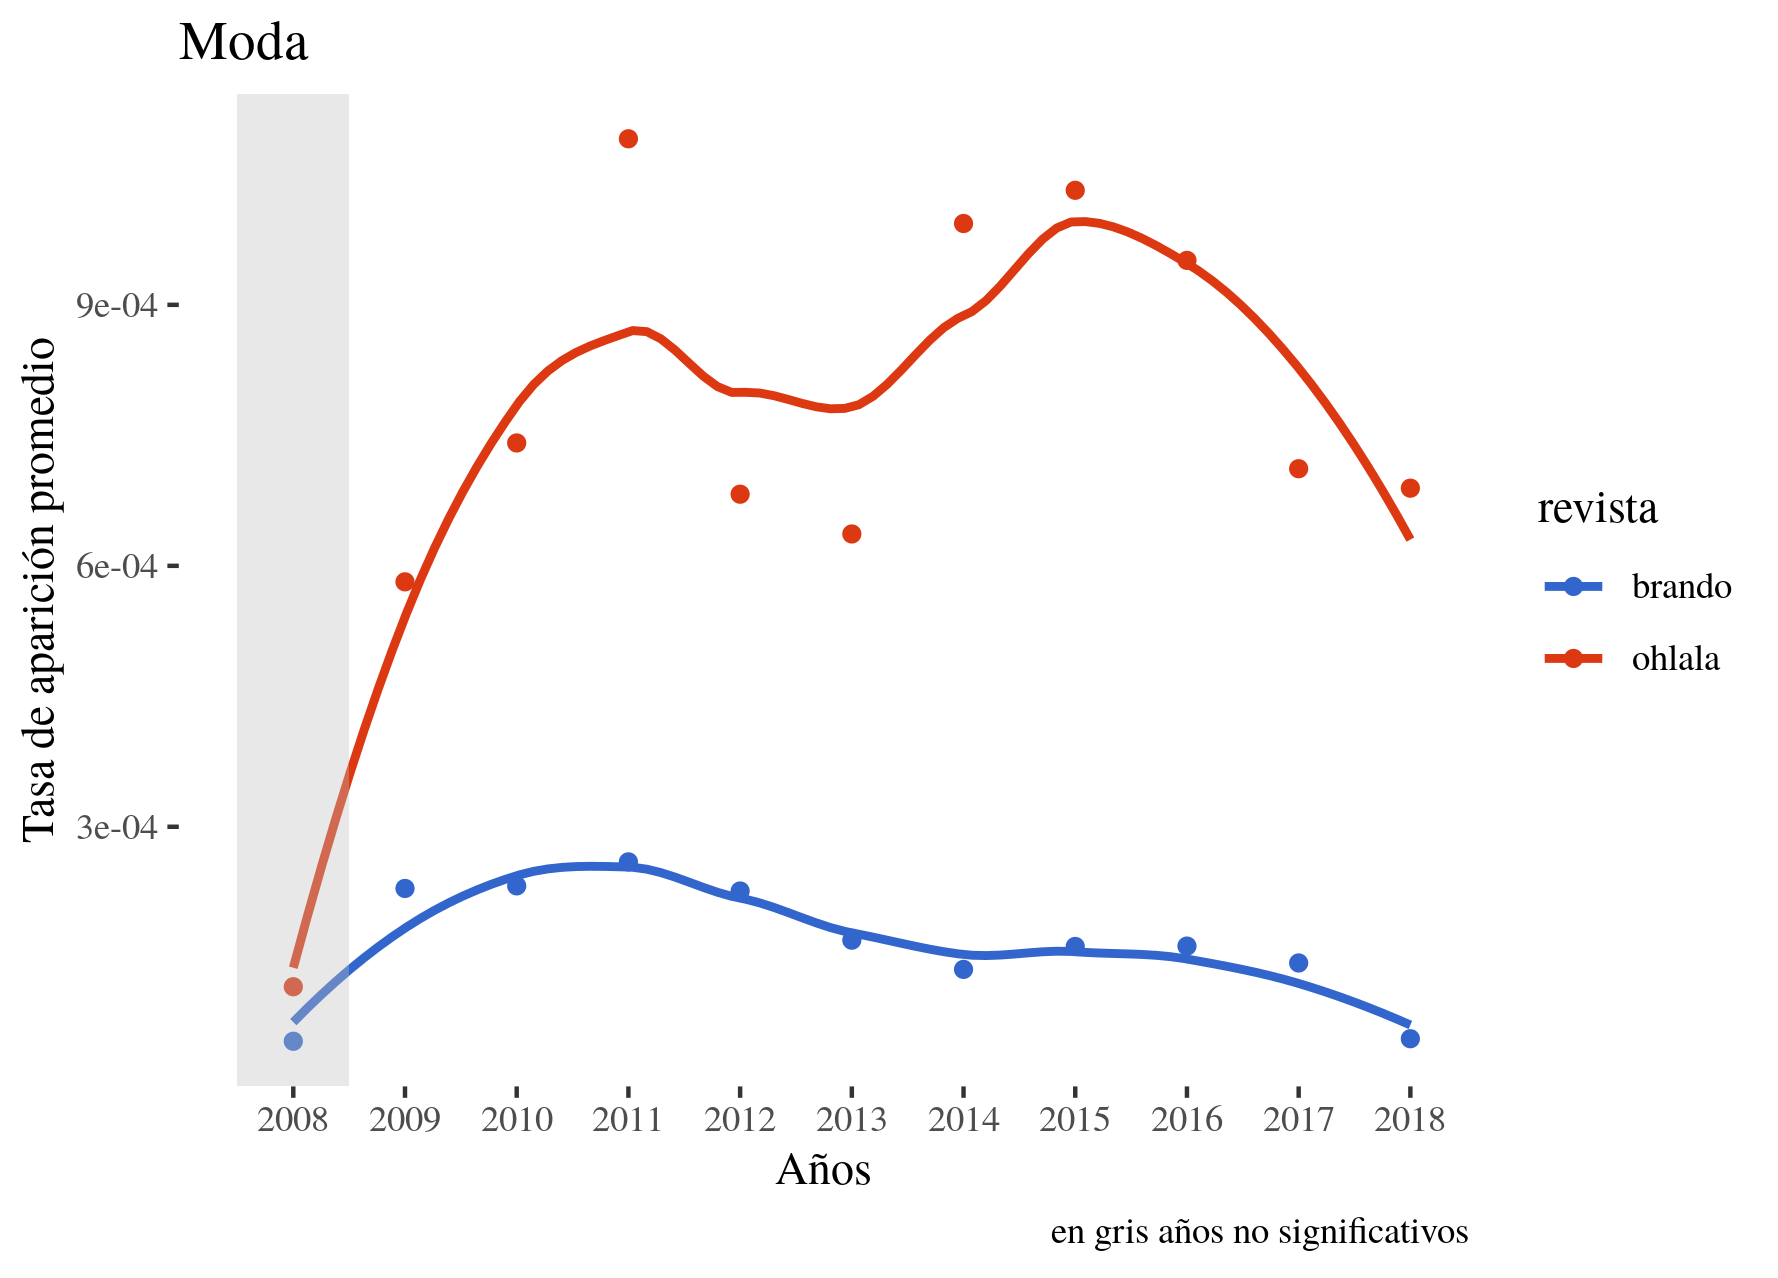
\includegraphics[width=65mm]{graficos/Moda.png}}
\subfigure[Tab\'ues]{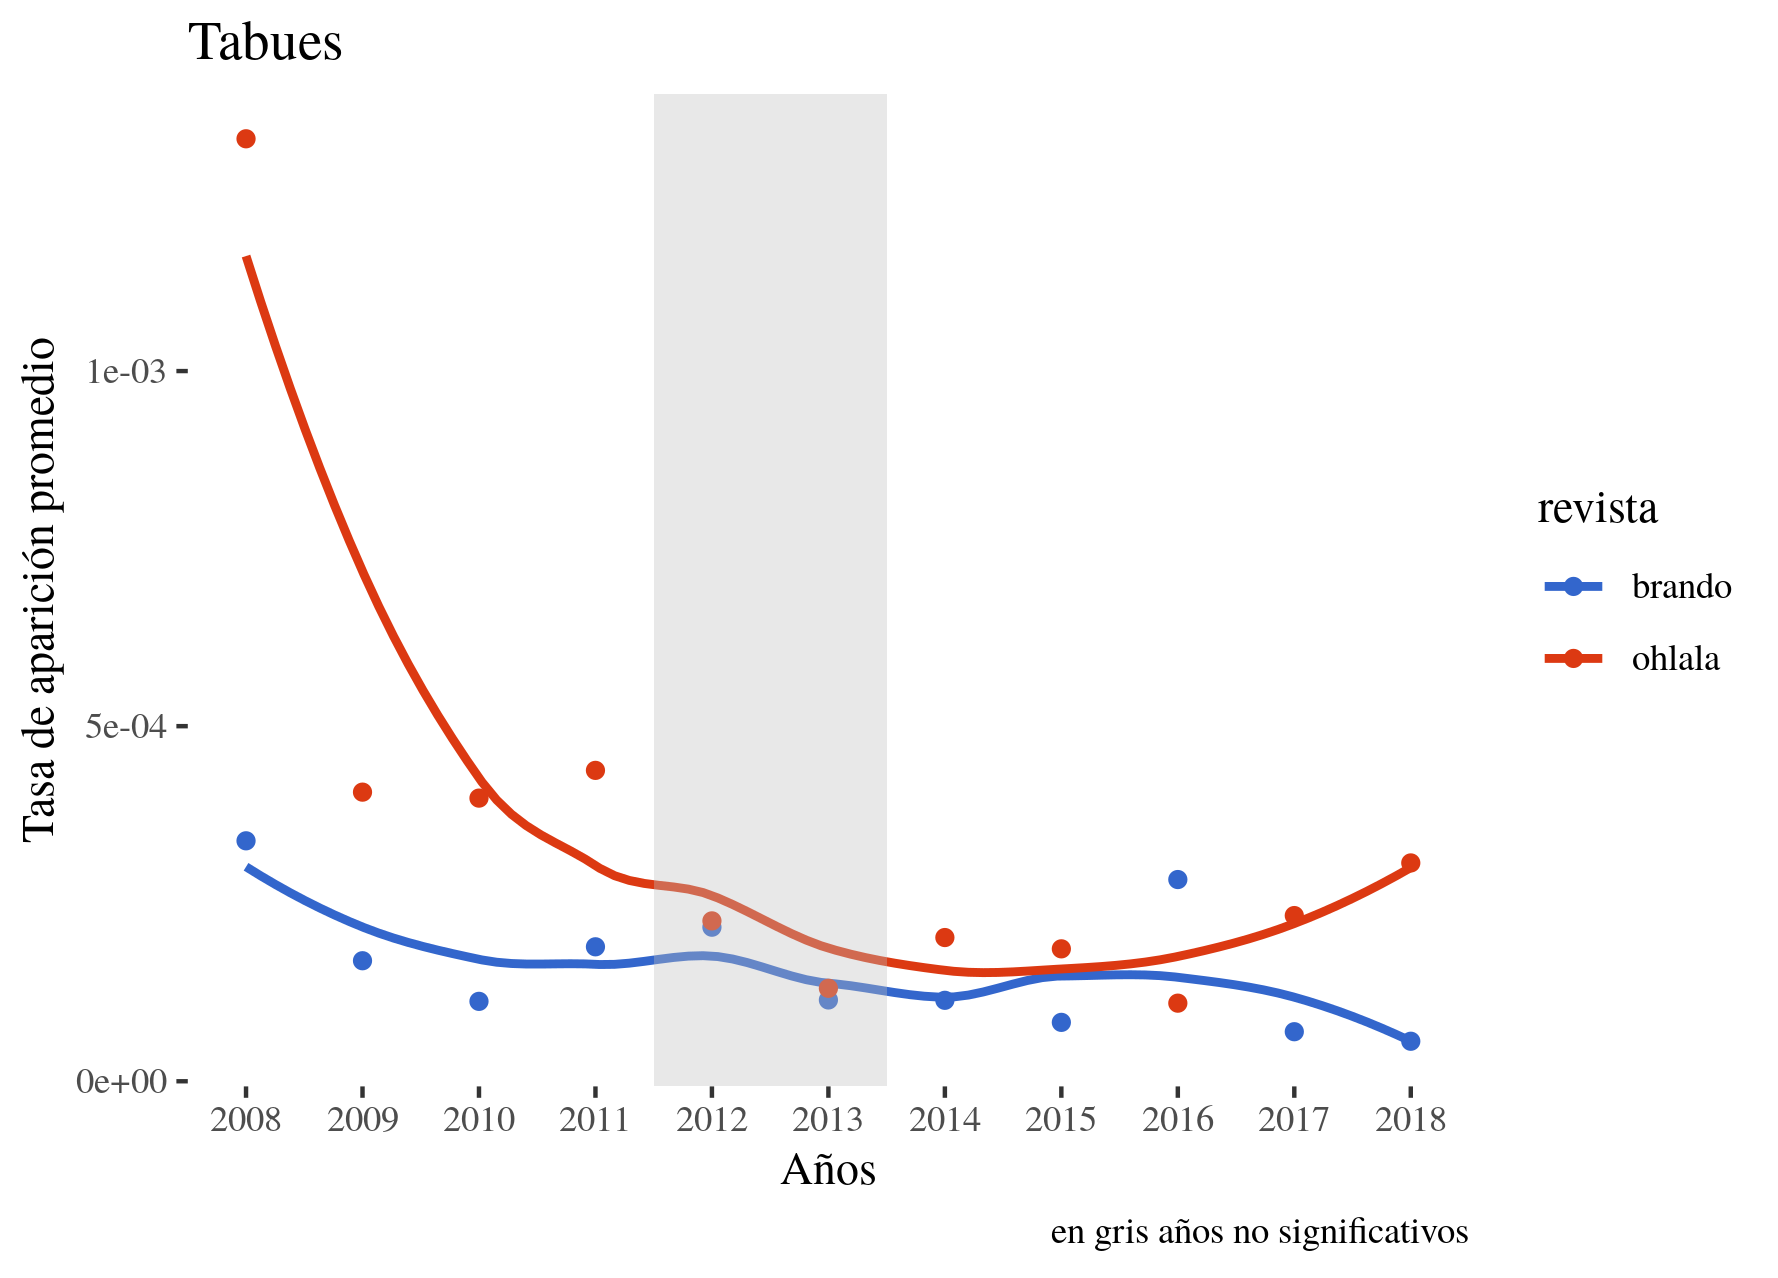
\includegraphics[width=65mm]{graficos/Tabues.png}}
\caption{Palabras relacionadas a Moda y Tab\'ues} \label{fig:modaytabu}
\end{figure}

Observando las palabras asociadas a \textbf{"Moda"} al contrario de lo observado en los gr\'aficos anteriores, vemos que son palabras mayormente utilizadas en la revista femenina. Excepto el a\~no 2008 las diferencias son siempre significativas.\\
Moda se mantiene siempre en niveles altos en Ohlala, y declinando en el tiempo en Brando pero us\'andolas en baja proporci\'on en esta \'ultima.

Las palabras sobre \textbf{"Tab\'ues"}, eran ampliamente usadas en Ohlala por sobre Brando en los primero a\~nos, y si bien se mantienen en mayor uso en dicha revista con diferencias significativas (excepto 2012, 2013 y 2016), los "gaps" son menores.

\begin{figure}[H]
\centering
\subfigure[Feminismo]{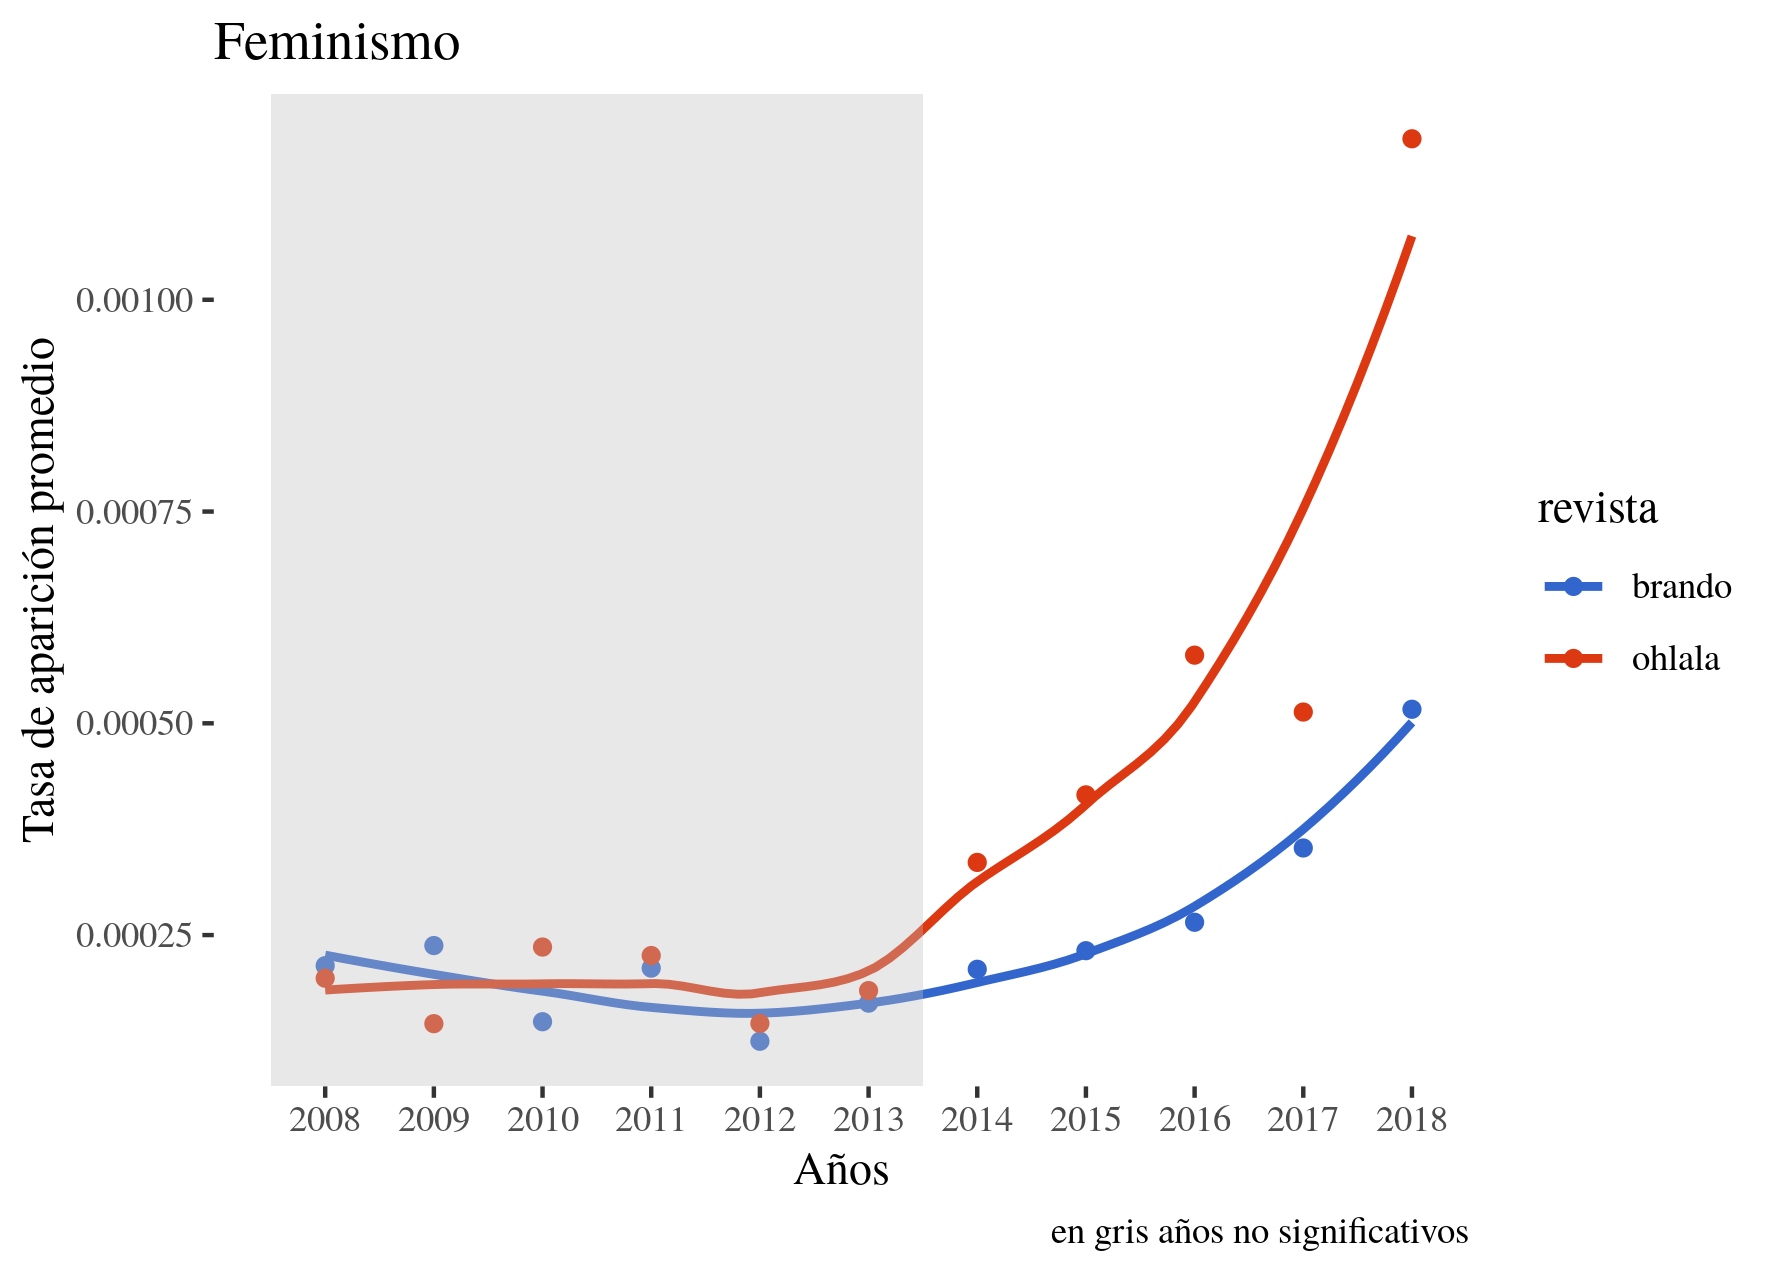
\includegraphics[width=65mm]{graficos/Feminismo.png}}
\subfigure[Sexista]{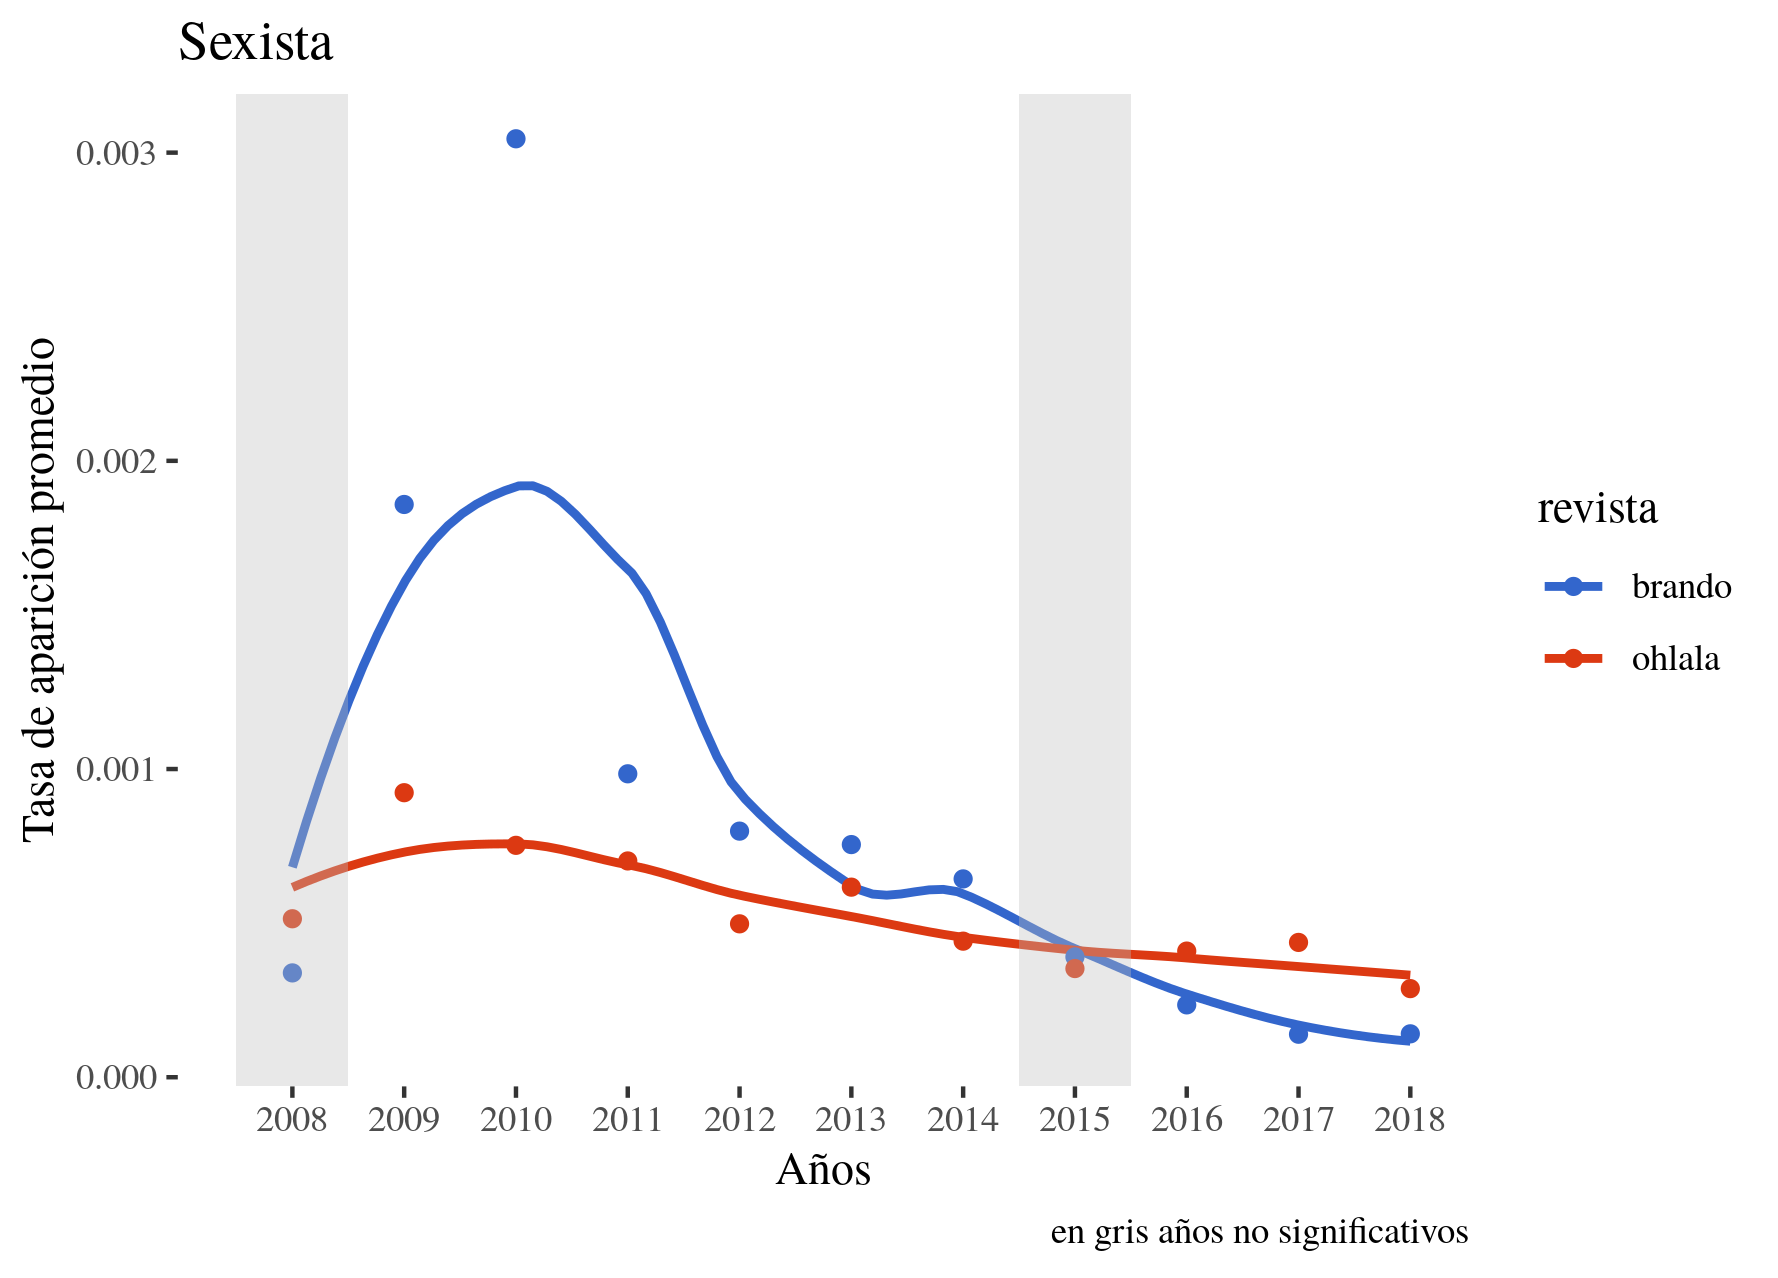
\includegraphics[width=65mm]{graficos/Sexista.png}}
\caption{Palabras relacionadas a Feminismo y Sexista} \label{fig:femysexista}
\end{figure}

Referido las palabras asociadas a \textbf{"Feminismo"} y \textbf{"Sexista"}, claramente notamos un cambio de comportamiento a lo largo de los a\~nos (H2).\\
Feminismo en los a\~nos iniciales se usa en bajas proporciones en ambas revistas y las diferencias son no significativas. Es a partir de 2014 que toman relevancia en ambas, aunque en mayor medida en Ohlala, seguramente relacionado a un cambio cultural.\\
Las palabras sexistas eran mayormente usadas en Brando, con diferencias significativas versus ohlala (excepto 2008 y 2015). Sin embargo en 2016 las curvas se cruzan y dichas palabras son usadas en mayor proporci\'on en ohlala. 


\begin{figure}[H]
\centering
\subfigure[Negocios]{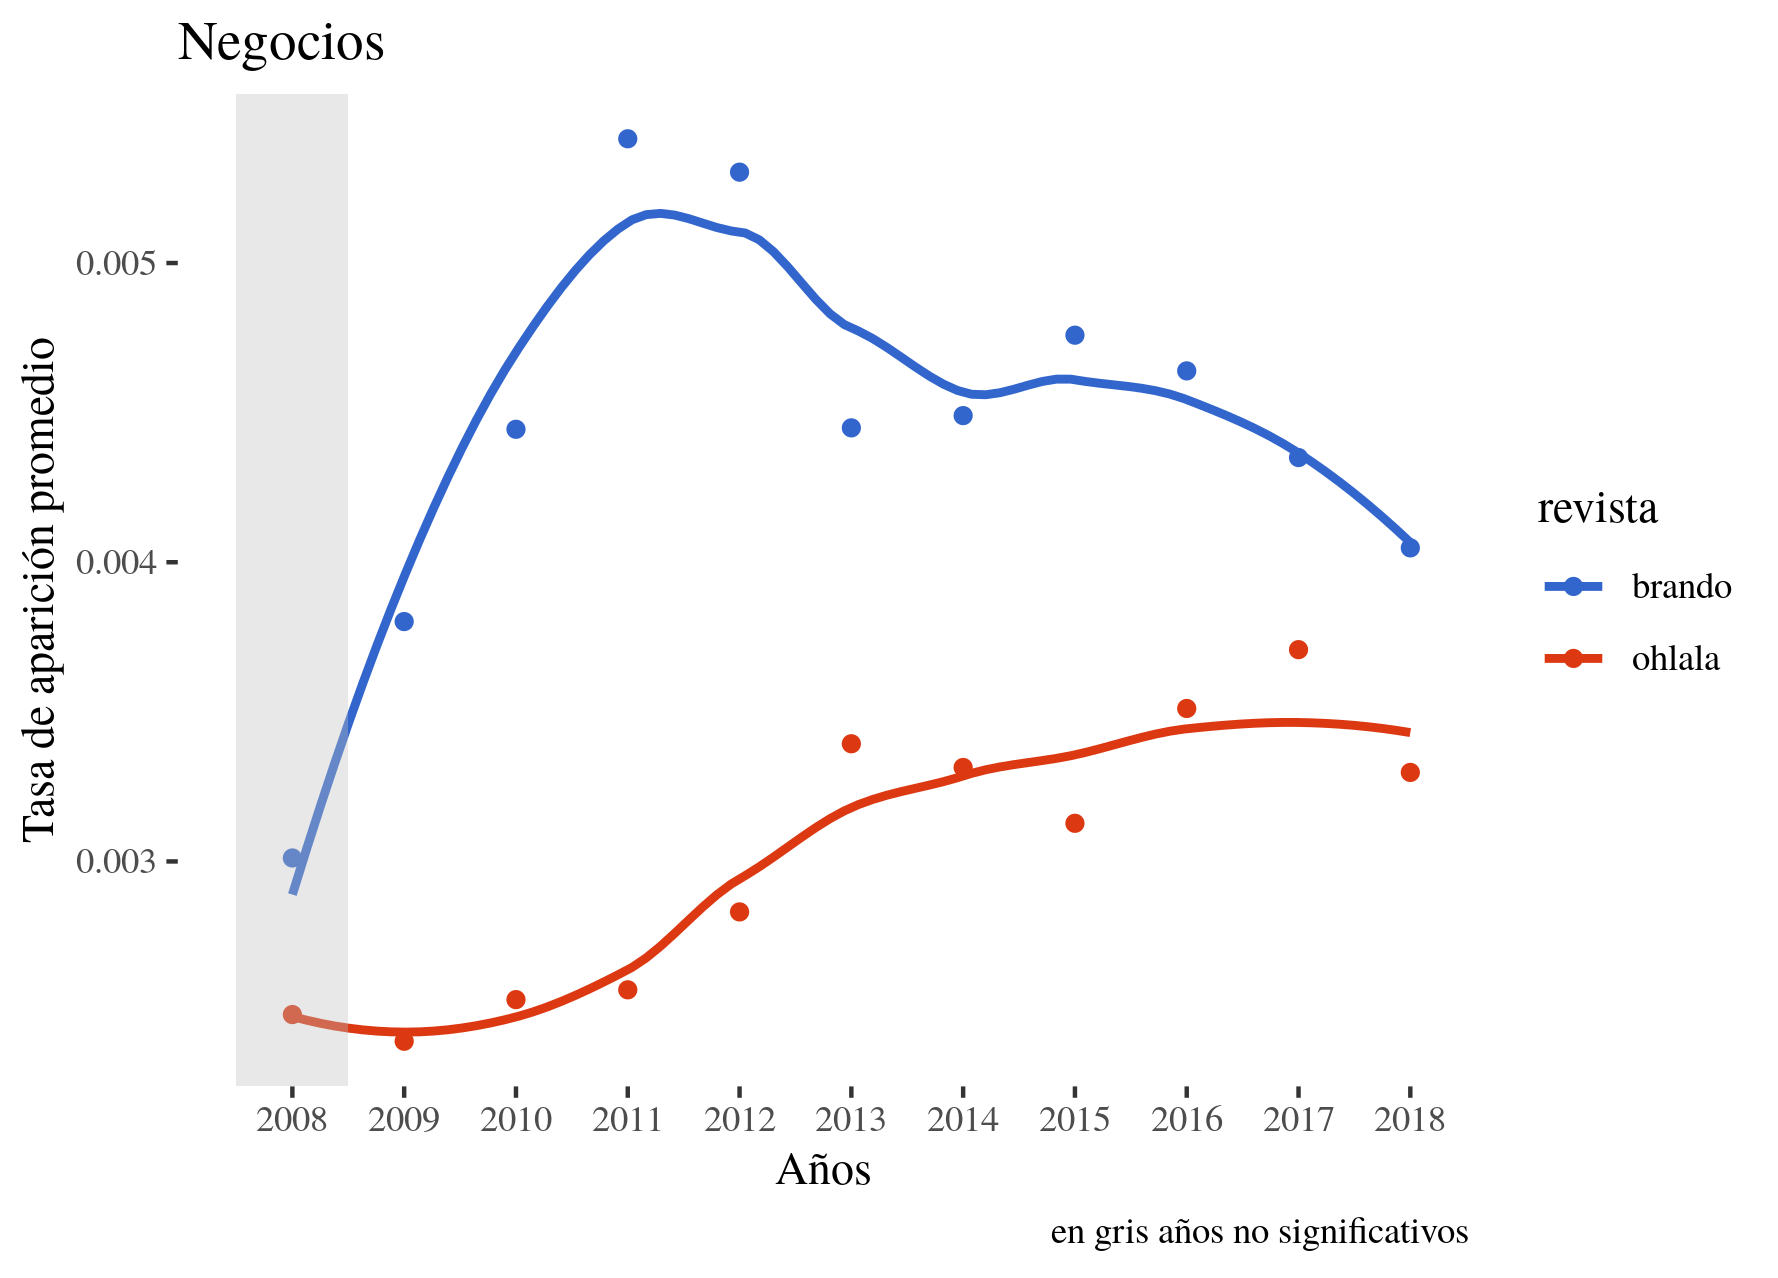
\includegraphics[width=65mm]{graficos/Negocios.png}}
\subfigure[Hor\'oscopo]{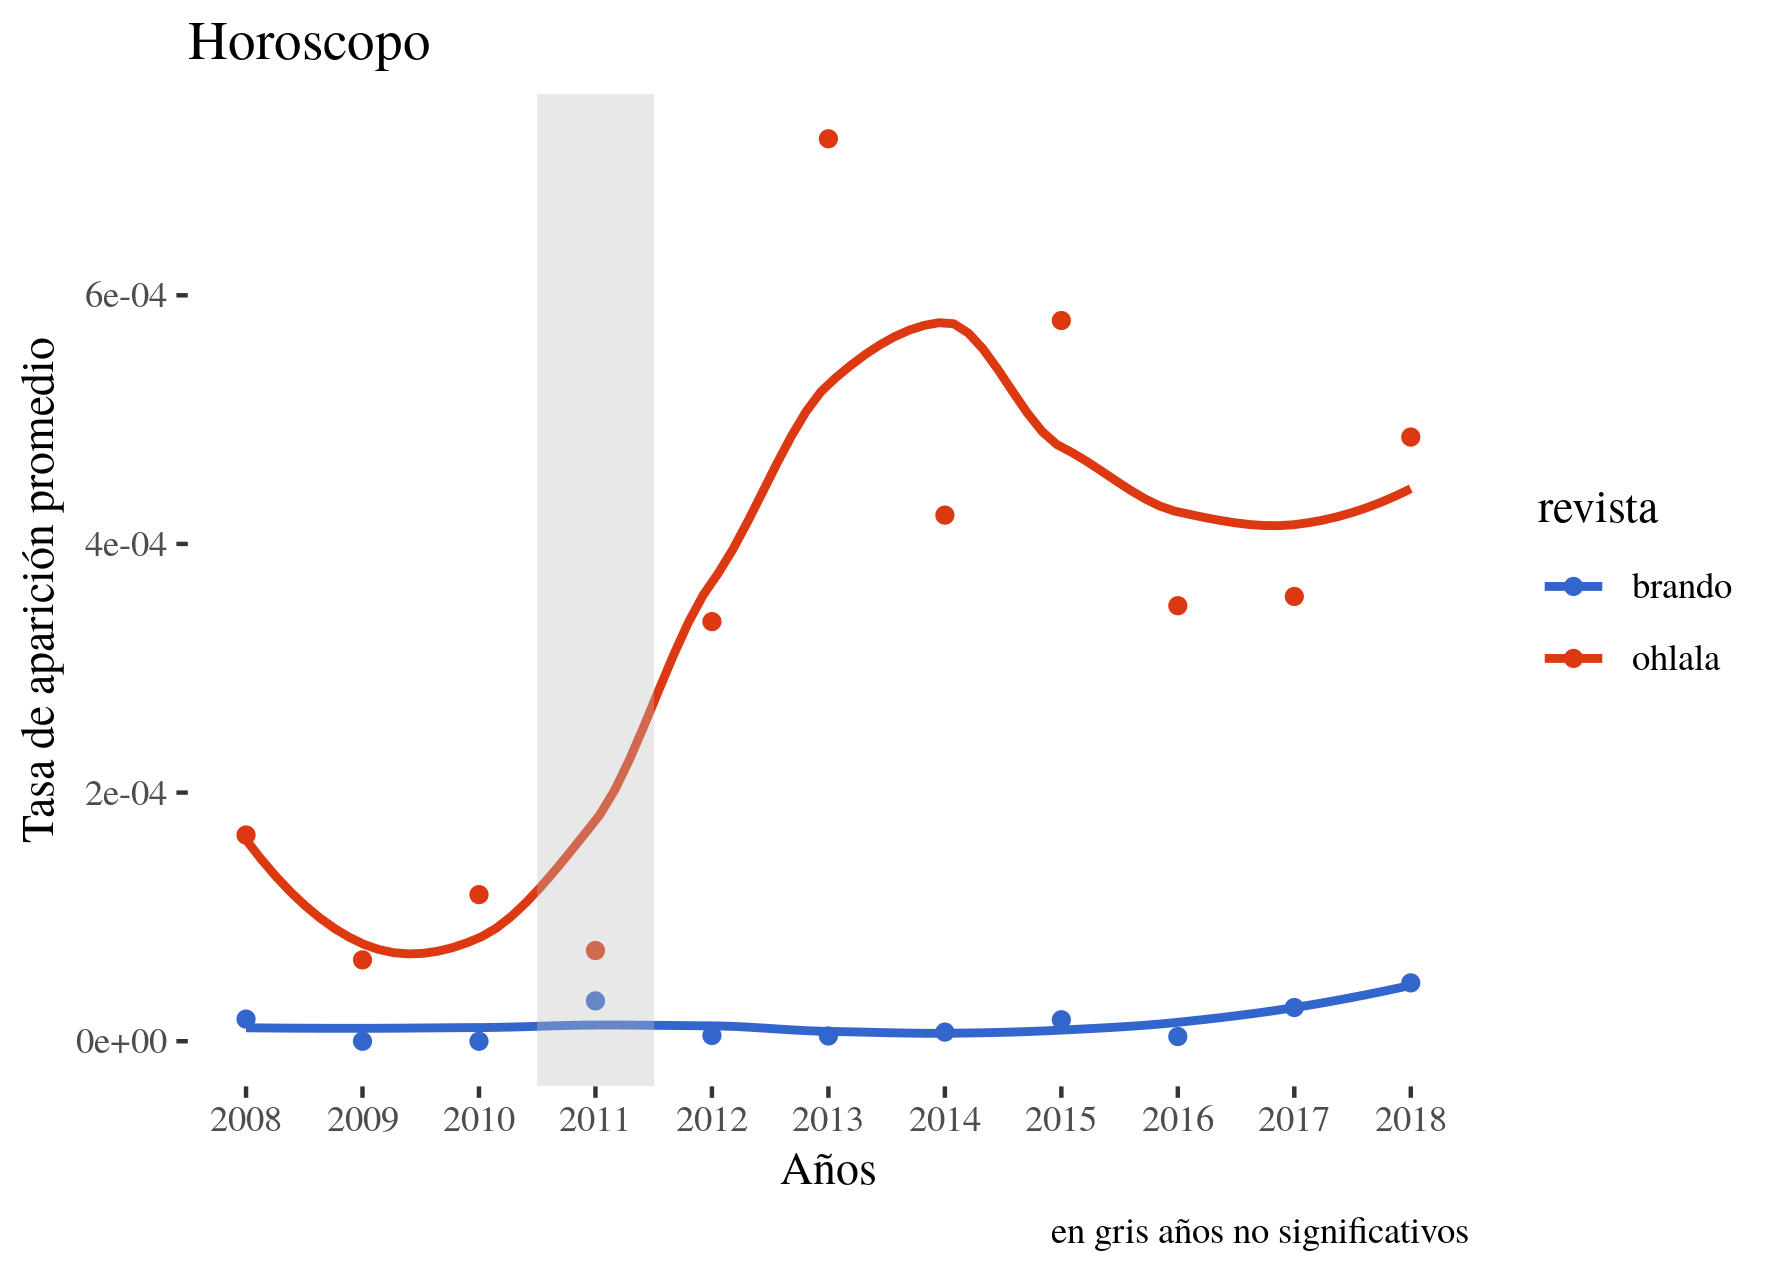
\includegraphics[width=65mm]{graficos/Horoscopo.png}}
\caption{Palabras relacionadas a Negocios y Hor\'oscopo} \label{fig:negoyhoro}
\end{figure}

Abordamos ahora las palabras asociadas a \textbf{"Negocios"} y \textbf{"Hor\'oscopo"}.\\
En Hor\'oscopo, excepto el a\~no 2011, las diferencias son siempre significativas y orientadas hacia el p\'ublico femenino. Inicia con niveles bajos de utilizaci\'on en Ohlala, aunque luego de 2011 se convierte en un tema recurrente en la magazine femenina.\\
Negocios en cambio (excepto 2008) siempre muestra diferencias significativas con clara orientaci\'on al p\'ublico masculino. Aunque tambi\'en, como ocurr\'ia en Ciencias, se devela un comportamiento ascendente en las proporciones de uso en ohlala, aunque siempre por debajo de Brando.\\
A partir de este \'ultimo an\'alisis podemos afirmar el cumplimiento de la H3 \textit{"Otros t\'opicos se mantienen en el tiempo, asignando roles aspiracionales diferenciados entre hombres y mujeres."} donde cit\'abamos los ejemplos que acabamos de tratar.


\section{Conclusiones}

A trav\'es de este trabajo de investigaci\'on pudimos abordar el objetivo general, analizando dos revistas de consumo masivo con orientaci\'on a p\'ublicos femenino y masculino, mediante de procesamiento de lenguaje.\\

Para el contraste de las hip\'otesis inicialmente planteadas utilizamos dos v\'ias de an\'alisis.\\
Mediante los t\'opicos pudimos comprobar que hay temas que usualmente son planteados desde las l\'ineas editoriales como propios del inter\'es de cada g\'enero. Tal es el caso de Autos, F\'utbol, Investigaci\'on, Negocios y Sociedad para los hombres, y Familia, Moda y Ni\~nos para las mujeres. Esto confirmar\'ia la Hip\'otesis 1.\\
En cuanto a la Hip\'otesis 2, not\'amos que temas como Familia y Ni\~nos, antes mayoritariamente orientados al p\'ublico femenino, con el pasar de los a\~nos fueron convirti\'endose en temas tratados por ambas editoriales, acorde al mayor rol asumido por el hombre en el seno familiar.\\
\linebreak
Analizando los Listados de Palabras, corroboramos que hay temas como Ciencia, Trendy y Negocios que son mayormente utilizados en la revista masculina, y otros como Hor\'oscopo y Moda en las femeninas.\\ M\'as all\'a de poder mostrar un inter\'es de hombres y mujeres a ciertos temas, tambi\'en es cierto que dichos temas son de inter\'es para el g\'enero opuesto, muchas veces con igual intensidad.\\
En cuanto a la hip\'otesis 2, con el listado de palabras Sexistas notamos claramente una evoluci\'on a la baja en su utilizaci\'on en la revista masculina, probablemente asociada a un cambio cultural.\\
Para destacar es el tema del Feminismo, donde a partir de 2014 se nota un amplio crecimiento en su proporci\'on de utilizaci\'on, acorde al surgimiento de fuerzas sociales tendientes a lograr la igualdad de trato y oportunidades para el colectivo femenino.\\
Con respecto a la hip\'otesis 3, corroboramos c\'omo el estereotipo de las l\'ineas editoriales tienden a hablarles de Negocios a los hombres, y del Hor\'oscopo a las mujeres. Suponemos que esto podr\'ia tener relaci\'on con un pensamiento de tintes machistas, donde es el hombre quien emprende y lidera los negocios, relegando a la mujer a un rol pasivo y librado a la suerte o destino.\\
Este trabajo puede servir de puntapi\'e inicial para futuras investigaciones que ampl\'ien el abanico de revistas de g\'enero analizadas, y que al ser de sumo inter\'es para la sociedad en general, puede servir para motivar las discusiones necesarias en este sentido.\\
\linebreak
Se puede acceder al material de este trabajo ingresando a trav\'es del link de github que contiene los c\'odigos y principales resultados obtenidos \cite{github}.


\bibliographystyle{plain}
\bibliography{sample}

\end{document}